% Metódy inžinierskej práce

\documentclass[10pt,oneside,english,a4paper]{article}

\usepackage[english]{babel}
%\usepackage[T1]{fontenc}
\usepackage[IL2]{fontenc} % lepšia sadzba písmena Ľ než v T1
\usepackage[utf8]{inputenc}
\usepackage{graphicx}
\usepackage{url} % príkaz \url na formátovanie URL
\usepackage[hidelinks]{hyperref} % odkazy v texte budú aktívne (pri niektorých triedach dokumentov spôsobuje posun textu)

\usepackage{cite}

\setlength\parindent{24pt}

\pagestyle{headings}

\title{Different types of Gamifications in Studying and their Effect on Motivation\thanks{Semester project of Engineering Methods class, ak. rok 2022/23, teacher: MSc. Mirwais Ahmadzai}} 

\author{Adam Candrák\\[2pt]
	{\small Slovenská technická univerzita v Bratislave}\\
	{\small Fakulta informatiky a informačných technológií}\\
	{\small \texttt{xcandrak@is.stuba.sk}}
	}

\date{\small 1.11.2022}



\begin{document}

\maketitle

\begin{abstract}
Interest in gamification in education is steadily rising the past few years due to its potential to increase the motivation and engagement of students. Yet, a large number of people are still far away from fully understanding the impact of gamification on students and/or are unaware of some types of gamification. Therefore, the purpose of this article is to highlight different ways of implementing game-like aspects in education and to compare these types and their strengths and weaknesses. Based on this information, we will suggest the most successful way to gamify a study programme.
\\\\
\textbf {Keywords} – Gamification, Studying, Motivation

\end{abstract}



\section{Introduction}


\par
All sorts of games are beginning to take root in our culture and are generally becoming more popular every day. From the current batch of Generation Z students, almost all students are already familiar with at least one type of computer game, and these games have become more and more integrated into their lives, opening the possibility of attracting their attention through engaging systems known to them. This possibility turns to almost a necessity due to the sanitary contingency of COVID-19 teachers and students of all countries were forced to isolate at their homes and work, study and live in just one place, decreasing motivation as the students have no designated place with the sole purpose of focusing on their tasks and learning.\cite{virtual}
\par
Furthermore, every students is different when it comes to their style of studying or their previously acquired skills. To address this problem diversified type of learning is required. Since accommodating every students in the class is a grueling task, gamification serves as new option for the learners.\cite{adaptive}
\par
Extensive research has been done on the topic of gamification by Lavoué, Hernández-Muñoz, Dicheva, Irwin, Kim, Lockee and many more.




\section{Game} \label{game}

\par
One of the most famous definitions of the term "game" comes from legendary game designer and producer Sid Meier, which states, “a game is a series of interesting and meaningful choices made by the player in pursuit of a clear and compelling goal.” It is hard to disagree with this statement, after all, many researchers agree with him.\cite{Hu:gamification}
\par
In the history, the term was commonly definition of the term was “an activity directed toward bringing about a specific state of affairs, using only means permitted by specific rules, where the means permitted by the rules are more limited in scope than they would be in the absence of the rules, and where the sole reason for accepting such limitation is to make possible such activity”.\cite{suits:game} Even now, the exact definition is unclear and debatable. 
\par 
However, certain characteristics of games are part of every definition. Characteristics such as goals, rules and feedback systems. This means that games are able to evoke extrinsic motivation in the player by establishing goals and immediately rewarding the player after achieving these goals. Furthermore, with the rules, players know what they need to do and what can occur within a game. Rules are usually defined before beginning a game, but some rules can be modified, created, or removed in concert with the player's skill level or other variables.\cite{Hu:gamification}


\subsection{Types of Games} \label{types of games}

\par
There are many types of games. Some focus on specific game types, while others focus on all games in general. The researcher Juul suggested that video games should also be classified. He argued that there are only five video game types: abstract, iconic, incoherent world, coherent world and staged games. Vossen argued that games should be specified based on three distinctions: competitiveness, interaction and if the game is physical or not. Based on this the researchers classified games into noncompetitive-nonphysical games, parallel-nonphysical games, interactive-nonphysical games, noncompetitive sports, parallel sports, and interactive sports. Based on these classifications Google has created a list of of categories for their app stores as shown in the Table. \cite{Hu:gamification} 
\par
The educational game genre is a game type that supports learners in acquiring knowledge, attitudes and skills on a specific topic. It is a game that also meets the educational purposes. Such games can be crosswords, solitaires, quizzes or chess just to name a few.
The simulation game genre is also an example of education in games, as these games simulate a real world or fictional situation that the player wouldn't be able to experience under normal circumstances. Such games are the Euro Truck Simulator, Farming Simulator or Microsoft's Flight Simulator just to name some of the popular ones. 
The strategy, trivia, puzzle and word games can also be used in certain situations for educational purposes.

\section{Flow Theory} \label{flow theory}

\par
The term Flow Theory was introduced into psychology by Csikszentmihalyi in 1975.\cite{1990flow} In this celebrated study, Csikszentmihalyi focused on highly performing individuals from a range of professions. While interviewing different people most of their descriptions of their optimal experience included a sense of effortless action, as if nothing else seemed to matter, and the experience itself was the whole.\cite{runco}
\par
Csikszentmihalyi’s research also revealed some counter-intuitive things about optimal experience. He found that many of the activities people pursue in their leisure time were among the least enjoyable. The most enjoyable moments were rather the ones full of challenge and even pain. However, too challenging activities lead to stress, frustration and anxiety and sometimes the individuals might even give up trying to perform said activities. On the other hand, if the activity is below the individual's skill level they feel bored. \\Figure \ref{flowstate}  illustrates the flow theory.
\par
These are four mental states: anxiety, apathy, boredom, and flow. From these states flow is the most optimal for learning as it increases focus and motivation. Therefore, in order to provide the best possible learning environment to every student challenges should require the highest level of their abilities. \cite{Hu:gamification}
\begin{figure}[h]
\caption{Csikszentmihalyi’s flow theory}
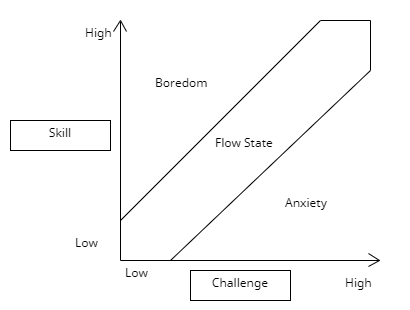
\includegraphics[scale=0.8]{Flowstate}
\label{flowstate}
\end{figure}





\section{Types of Gamification} \label{gamification}



\section{Conclusion} \label{Conclusion} 



\bibliography{bibliography}
\bibliographystyle{plain} % prípadne alpha, abbrv alebo hociktorý iný
\end{document}
